% fit-md-field-theory.tex
\documentclass[tikz]{standalone}
\usepackage{amsmath}
\usepackage{amssymb}
\usepackage{graphicx}
\usepackage{pgfplots}
\usepackage[dvipsnames]{xcolor}
\usetikzlibrary{arrows.meta}
\pgfplotsset{compat=1.18} % or your preferred version

\newcommand{\drawGrid}[5]{% #1=xmin, #2=ymin, #3=xmax, #4=ymax, #5=spacing
  \begingroup
  % ensure numeric evaluation
  \pgfmathsetmacro{\DGxmin}{#1}%
  \pgfmathsetmacro{\DGxmax}{#3}%
  \pgfmathsetmacro{\DGymin}{#2}%
  \pgfmathsetmacro{\DGymax}{#4}%
  \pgfmathsetmacro{\DGdx}{#5}%
  % guard against zero/negative spacing
  \pgfmathparse{abs(\DGdx)>0 ? \DGdx : 1} \let\DGdx\pgfmathresult
  % compute number of steps (cover up to xmax/ymax)
  \pgfmathsetmacro{\DGnVert}{ceil((\DGxmax-\DGxmin)/\DGdx)}%
  \pgfmathtruncatemacro{\DGNV}{\DGnVert}%
  \pgfmathsetmacro{\DGnHorz}{ceil((\DGymax-\DGymin)/\DGdx)}%
  \pgfmathtruncatemacro{\DGNH}{\DGnHorz}%
  \begin{scope}
    % Use axis coordinates when inside an axis; safe outside too
    \clip (axis cs:\DGxmin,\DGymin) rectangle (axis cs:\DGxmax,\DGymax);
    % vertical lines
    \foreach \DGi in {0,...,\DGNV} {%
      \pgfmathsetmacro{\DGxcoord}{\DGxmin + \DGi*\DGdx}%
      \draw[gray!50,thin] (axis cs:\DGxcoord,\DGymin) -- (axis cs:\DGxcoord,\DGymax);%
    }%
    % horizontal lines
    \foreach \DGj in {0,...,\DGNH} {%
      \pgfmathsetmacro{\DGycoord}{\DGymin + \DGj*\DGdx}%
      \draw[gray!50,thin] (axis cs:\DGxmin,\DGycoord) -- (axis cs:\DGxmax,\DGycoord);%
    }%
  \end{scope}
  \endgroup
}

\newcommand{\dg}[5]{
    
}

\begin{document}

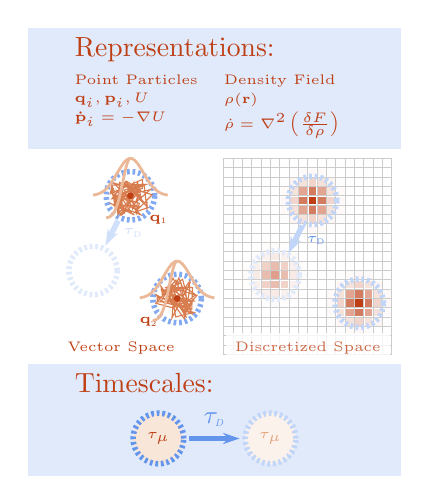
\begin{tikzpicture}
    \pgfmathsetmacro{\xmin}{-5}
    \pgfmathsetmacro{\xmax}{5}
    \pgfmathsetmacro{\ymin}{-6}
    \pgfmathsetmacro{\ymax}{6}
    
    \begin{axis}[
        axis lines=none,
        xmin=\xmin, xmax=\xmax,
        ymin=\ymin, ymax=\ymax,
        unit vector ratio=1 1,
        xtick=\empty, ytick=\empty
    ]

        % Draw fake boundary
        \pgfplotsextra{
            \path (axis cs:\xmin,\ymin) rectangle (axis cs:\xmax,\ymax);
        }

        % Draw shaded header / footer regions
        \pgfmathsetmacro{\yheader}{2.75}
        \pgfplotsextra{%
            \fill[CornflowerBlue!20, draw=none]
                (axis cs:\xmin,\ymax) rectangle (axis cs:\xmax,\yheader);
        }%

        \pgfmathsetmacro{\yfooter}{-3}
        \pgfplotsextra{%
            \fill[CornflowerBlue!20, draw=none]
                (axis cs:\xmin,\yfooter) rectangle (axis cs:\xmax,\ymin);
        }%

        % Draw particles in Vector Space
        \pgfmathsetmacro{\qxInit}{-2.25}
        \pgfmathsetmacro{\qyInit}{1.5}
        \pgfmathsetmacro{\qxFinal}{-3.25}
        \pgfmathsetmacro{\qyFinal}{-0.5}
        \pgfmathsetmacro{\qqx}{-1}
        \pgfmathsetmacro{\qqy}{-1.25}
        
        \pgfmathsetmacro{\qRadius}{0.65}
        
        \pgfplotsextra{%
          % draw two circular paths in axis coordinates (radius in axis units)
          \begin{scope}
            \draw[draw=CornflowerBlue!80, line width=2pt, dashed, dash pattern=on 1pt off 1pt, fill=none]
              (axis cs:\qxInit,\qyInit) ellipse ({\qRadius} and {\qRadius});
            \draw[draw=CornflowerBlue!80, line width=2pt, dashed, dash pattern=on 1pt off 1pt, fill=none]
              (axis cs:\qqx,\qqy) ellipse ({\qRadius} and {\qRadius});
            \draw[draw=CornflowerBlue!20, line width=2pt, dashed, dash pattern=on 1pt off 1pt, fill=none]
              (axis cs:\qxFinal,\qyFinal) ellipse ({\qRadius} and {\qRadius});

            % thick CornflowerBlue arrow pointing to the right-hand node
            \draw[line width=2pt, draw=CornflowerBlue!30, -{Stealth[length=6pt,width=4pt]}, shorten <=10pt, shorten >=10pt]
              (axis cs:\qxInit,\qyInit) -- (axis cs:\qxFinal,\qyFinal) node[pos=0.5, anchor=west, CornflowerBlue!30] {\tiny $\tau_{\scalebox{0.6}{D}}$};
          \end{scope}
        }%

        % Draw particles at q1, q2.
        % Add a Brownian path to Vector Space
        \pgfmathsetseed{1234} % reproducible

        % Path for q1
        % Initialize empty coordinate list
        \edef\coordlist{}
        
        \foreach \i in {1,...,60} {
            \pgfmathsetmacro{\theta}{rand*360}
            \pgfmathsetmacro{\r}{\qRadius*0.9*exp(-pow(rand,2))}
            \pgfmathsetmacro{\x}{\r*cos(\theta)}
            \pgfmathsetmacro{\y}{\r*sin(\theta)}
            \xdef\coordlist{\coordlist (\x+\qxInit,\y+\qyInit)}
        }
        
        % Plot all points as a connected path
        \addplot[Bittersweet!60, thin] coordinates {\coordlist};

        % Add particle as circle mark
        % point
        \addplot[
          Bittersweet,
          only marks,
          mark=*,
          mark options={scale=0.5, draw=Bittersweet, fill=Bittersweet},
        ] coordinates {(\qxInit,\qyInit)};

        % manual label placed with axis-unit offsets
        \node[Bittersweet, anchor=north west] 
          at (axis cs:{\qxInit+0.25},{\qyInit-0.25}) {\tiny$\mathbf{q}_{\scalebox{0.6}{1}}$};

        % Path for q2
        % Initialize empty coordinate list
        \edef\coordlist{}
        
        \foreach \i in {1,...,60} {
            \pgfmathsetmacro{\theta}{rand*360}
            \pgfmathsetmacro{\r}{\qRadius*0.9*exp(-pow(rand,2))}
            \pgfmathsetmacro{\x}{\r*cos(\theta)}
            \pgfmathsetmacro{\y}{\r*sin(\theta)}
            \xdef\coordlist{\coordlist (\x+\qqx,\y+\qqy)}
        }
        
        % Plot all points as a connected path
        \addplot[Bittersweet!60, thin] coordinates {\coordlist};

        % Add particle as circle mark
        % point
        \addplot[
          Bittersweet,
          only marks,
          mark=*,
          mark options={scale=0.5, draw=Bittersweet, fill=Bittersweet},
        ] coordinates {(\qqx,\qqy)};

        % manual label placed with axis-unit offsets
        \node[Bittersweet, anchor=north east] 
          at (axis cs:{\qqx-0.25},{\qqy-0.25}) {\tiny$\mathbf{q}_{\scalebox{0.6}{2}}$};
        
        % Draw a Gaussians around q1, q2
        \pgfmathsetmacro{\gaussianCenterX}{\qxInit}
        \pgfmathsetmacro{\gaussianBaseY}{\qyInit}
        \addplot [
            domain=\gaussianCenterX-1:\gaussianCenterX+1,
            samples=100,
            color=Bittersweet!30,
            line width=1pt,
            ]{1.0*exp(-4*(x-\gaussianCenterX)^2)+\gaussianBaseY};
        \addplot [
            domain=\gaussianCenterX-0.65:\gaussianCenterX,
            samples=100,
            color=Bittersweet!30,
            line width=1pt,
            ]{1.60*exp(-12*(x-\gaussianCenterX)^2)+\gaussianBaseY-.6};

        \pgfmathsetmacro{\gaussianCenterX}{\qqx}
        \pgfmathsetmacro{\gaussianBaseY}{\qqy}
        \addplot [
            domain=\gaussianCenterX-1:\gaussianCenterX+1,
            samples=100,
            color=Bittersweet!30,
            line width=1pt,
            ]{1.0*exp(-4*(x-\gaussianCenterX)^2)+\gaussianBaseY};
        \addplot [
            domain=\gaussianCenterX-0.65:\gaussianCenterX,
            samples=100,
            color=Bittersweet!30,
            line width=1pt,
            ]{1.60*exp(-12*(x-\gaussianCenterX)^2)+\gaussianBaseY-.6};

        % Draw grid
        \pgfmathsetmacro{\gridSpacing}{0.25}
        \pgfmathsetmacro{\gridXMin}{\gridSpacing}
        \pgfmathsetmacro{\gridSpacingXtwo}{\gridSpacing*2}
        \pgfmathsetmacro{\gridXMax}{\xmax-\gridSpacing}

        \pgfmathsetmacro{\gridYMin}{\yfooter+\gridSpacing}
        \pgfmathsetmacro{\gridSpacingYtwo}{\gridYMin+\gridSpacing}
        \pgfmathsetmacro{\gridYMax}{\yheader-\gridSpacing}

        \foreach \xValue in {\gridXMin,\gridSpacingXtwo,...,\gridXMax} {
            \addplot[black!20, thin] coordinates {(\xValue, \gridYMin) (\xValue, \gridYMax)};
        }
        \foreach \yValue in {\gridYMin,\gridSpacingYtwo,...,\gridYMax} {
            \addplot[black!20, thin] coordinates {(\gridXMin, \yValue) (\gridXMax, \yValue)};
        }

        % Plot Gaussian density
        \pgfmathsetmacro{\fieldqx}{\qxInit + \xmax}
        \pgfmathsetmacro{\fieldqy}{\qyInit}
        \pgfplotsextra{%
          \foreach \xi in {-3,...,3} {%
            \pgfmathsetmacro{\xx}{\xi*0.25}%
            \foreach \yi in {-3,...,3} {%
              \pgfmathsetmacro{\yy}{\yi*0.25}%
              \pgfmathsetmacro{\rr}{\xx*\xx + \yy*\yy}%
              \pgfmathsetmacro{\opacity}{exp(-6 * \rr)}% numeric between 0 and 1
              \pgfmathsetmacro{\xL}{\xx + \fieldqx - 0.125 - 0.1}%
              \pgfmathsetmacro{\xR}{\xx + \fieldqx - 0.125 + 0.1}%
              \pgfmathsetmacro{\yB}{\yy + \fieldqy - 0.125 - 0.1}%
              \pgfmathsetmacro{\yT}{\yy + \fieldqy - 0.125 + 0.1}%
              \draw[fill=Bittersweet!100, fill opacity=\opacity, draw=none]%
                (axis cs:\xL,\yB) rectangle (axis cs:\xR,\yT);%
            }%
          }%
        }%
        \draw[draw=CornflowerBlue!40, line width=2pt, dashed, dash pattern=on 1pt off 1pt, fill=none]
          (axis cs:\fieldqx-0.125,\fieldqy-0.125) ellipse ({\qRadius} and {\qRadius});

        \pgfmathsetmacro{\fieldqqx}{\qqx + \xmax}
        \pgfmathsetmacro{\fieldqqy}{\qqy}
        \pgfplotsextra{%
          \foreach \xi in {-3,...,3} {%
            \pgfmathsetmacro{\xx}{\xi*0.25}%
            \foreach \yi in {-3,...,3} {%
              \pgfmathsetmacro{\yy}{\yi*0.25}%
              \pgfmathsetmacro{\rr}{\xx*\xx + \yy*\yy}%
              \pgfmathsetmacro{\opacity}{exp(-6 * \rr)}% numeric between 0 and 1
              \pgfmathsetmacro{\xL}{\xx + \fieldqqx - 0.125 - 0.1}%
              \pgfmathsetmacro{\xR}{\xx + \fieldqqx - 0.125 + 0.1}%
              \pgfmathsetmacro{\yB}{\yy + \fieldqqy - 0.125 - 0.1}%
              \pgfmathsetmacro{\yT}{\yy + \fieldqqy - 0.125 + 0.1}%
              \draw[fill=Bittersweet!100, fill opacity=\opacity, draw=none]%
                (axis cs:\xL,\yB) rectangle (axis cs:\xR,\yT);%
            }%
          }%
        }%
        \draw[draw=CornflowerBlue!40, line width=2pt, dashed, dash pattern=on 1pt off 1pt, fill=none]
          (axis cs:\fieldqqx-0.125,\fieldqqy-0.125) ellipse ({\qRadius} and {\qRadius});

        \pgfmathsetmacro{\fieldqqxf}{\qxFinal + \xmax}
        \pgfmathsetmacro{\fieldqqyf}{\qyFinal}
        \pgfplotsextra{%
          \foreach \xi in {-3,...,3} {%
            \pgfmathsetmacro{\xx}{\xi*0.25}%
            \foreach \yi in {-3,...,3} {%
              \pgfmathsetmacro{\yy}{\yi*0.25}%
              \pgfmathsetmacro{\rr}{\xx*\xx + \yy*\yy}%
              \pgfmathsetmacro{\opacity}{exp(-6 * \rr)/2}% numeric between 0 and 1
              \pgfmathsetmacro{\xL}{\xx + \fieldqqxf - 0.125 - 0.1}%
              \pgfmathsetmacro{\xR}{\xx + \fieldqqxf - 0.125 + 0.1}%
              \pgfmathsetmacro{\yB}{\yy + \fieldqqyf - 0.125 - 0.1}%
              \pgfmathsetmacro{\yT}{\yy + \fieldqqyf - 0.125 + 0.1}%
              \draw[fill=Bittersweet!100, fill opacity=\opacity, draw=none]%
                (axis cs:\xL,\yB) rectangle (axis cs:\xR,\yT);%
            }%
          }%
        }%
        \draw[draw=CornflowerBlue!20, line width=2pt, dashed, dash pattern=on 1pt off 1pt, fill=none]
          (axis cs:\fieldqqxf-0.125,\fieldqqyf-0.125) ellipse ({\qRadius} and {\qRadius});
          
        % thick CornflowerBlue arrow pointing to the right-hand node
        \draw[line width=2pt, draw=CornflowerBlue!40, -{Stealth[length=6pt,width=4pt]}, shorten <=12pt, shorten >=7pt]
          (axis cs:\fieldqx,\fieldqy) -- (axis cs:\fieldqqxf,\fieldqqyf) node[pos=0.6, anchor=west, CornflowerBlue] {\tiny $\tau_{\scalebox{0.6}{D}}$};

        % Representations legend
        \node[anchor=north west, color=Bittersweet] at (axis cs:-4,6) {Representations:};
    
        \node[anchor=north west, color=Bittersweet] at (axis cs:-4,5) {\tiny Point Particles};
        \node[anchor=north west, color=Bittersweet] at (axis cs:-4,4.5) {\tiny $\mathbf{q}_i, \mathbf{p}_i, U$};
        \node[anchor=north west, color=Bittersweet] at (axis cs:-4,4) {\tiny $\mathbf{\dot{p}}_i = - \nabla U$};
    
        \node[anchor=north west, color=Bittersweet] at (axis cs:0,5) {\tiny Density Field};
        \node[anchor=north west, color=Bittersweet] at (axis cs:0,4.5) {\tiny $\rho(\mathbf{r})$};
        \node[anchor=north west, color=Bittersweet] at (axis cs:0,4) {\tiny $\dot{\rho} = \nabla^2 \left(\frac{\delta F}{\delta \rho}\right)$};

        % Space labels
        \node[anchor=north, color=Bittersweet] at (axis cs:\xmin/2,\yfooter+0.85) {\tiny Vector Space};
        \node[anchor=north, color=Bittersweet, fill=white, fill opacity=0.8] at (axis cs:\xmax/2,\yfooter+0.85) {\tiny Discretized Space};
    
        % Timescales legend
        \node[anchor=north west, color=Bittersweet] at (axis cs:-4,-3) {Timescales:};
        
        % original (make it a named node)
        \node[name=labelA, circle, anchor=south, color=Bittersweet, draw=CornflowerBlue, line width=2pt, dashed, dash pattern=on 1pt off 1pt, align=center, fill=Bittersweet!10] 
          at (axis cs:-1.5,-5.75) {\tiny $\tau_\mu$};
        
        % lighter copy shifted to the right (adjust xshift as needed)
        \node[name=labelB, circle, anchor=south, color=Bittersweet!40, draw=CornflowerBlue!40, line width=2pt, dashed, dash pattern=on 1pt off 1pt, align=center, fill=Bittersweet!5] 
          at (axis cs:+1.5,-5.75) {\tiny $\tau_\mu$};
        
        % thick CornflowerBlue arrow pointing to the right-hand node
        \draw[line width=2pt, draw=CornflowerBlue, -{Stealth[length=6pt,width=4pt]}, shorten >=1pt, shorten <=1pt]
          (labelA.east) -- (labelB.west) node[midway, above, CornflowerBlue] {\small $\tau_{\scalebox{0.4}{$D$}}$};
      
    \end{axis}
    
\end{tikzpicture}

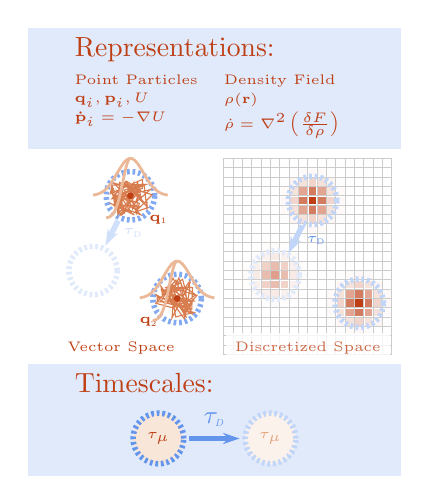
\begin{tikzpicture}
    \pgfmathsetmacro{\xmin}{-5}
    \pgfmathsetmacro{\xmax}{5}
    \pgfmathsetmacro{\ymin}{-6}
    \pgfmathsetmacro{\ymax}{6}
    
    \begin{axis}[
        axis lines=none,
        xmin=\xmin, xmax=\xmax,
        ymin=\ymin, ymax=\ymax,
        unit vector ratio=1 1,
        xtick=\empty, ytick=\empty
    ]

        % Draw fake boundary
        \pgfplotsextra{
            \path (axis cs:\xmin,\ymin) rectangle (axis cs:\xmax,\ymax);
        }

        % Draw shaded header / footer regions
        \pgfmathsetmacro{\yheader}{2.75}
        \pgfplotsextra{%
            \fill[CornflowerBlue!20, draw=none]
                (axis cs:\xmin,\ymax) rectangle (axis cs:\xmax,\yheader);
        }%

        \pgfmathsetmacro{\yfooter}{-3}
        \pgfplotsextra{%
            \fill[CornflowerBlue!20, draw=none]
                (axis cs:\xmin,\yfooter) rectangle (axis cs:\xmax,\ymin);
        }%

        % Draw particles in Vector Space
        \pgfmathsetmacro{\qxInit}{-2.25}
        \pgfmathsetmacro{\qyInit}{1.5}
        \pgfmathsetmacro{\qxFinal}{-3.25}
        \pgfmathsetmacro{\qyFinal}{-0.5}
        \pgfmathsetmacro{\qqx}{-1}
        \pgfmathsetmacro{\qqy}{-1.25}
        
        \pgfmathsetmacro{\qRadius}{0.65}
        
        \pgfplotsextra{%
          % draw two circular paths in axis coordinates (radius in axis units)
          \begin{scope}
            \draw[draw=CornflowerBlue!80, line width=2pt, dashed, dash pattern=on 1pt off 1pt, fill=none]
              (axis cs:\qxInit,\qyInit) ellipse ({\qRadius} and {\qRadius});
            \draw[draw=CornflowerBlue!80, line width=2pt, dashed, dash pattern=on 1pt off 1pt, fill=none]
              (axis cs:\qqx,\qqy) ellipse ({\qRadius} and {\qRadius});
            \draw[draw=CornflowerBlue!20, line width=2pt, dashed, dash pattern=on 1pt off 1pt, fill=none]
              (axis cs:\qxFinal,\qyFinal) ellipse ({\qRadius} and {\qRadius});

            % thick CornflowerBlue arrow pointing to the right-hand node
            \draw[line width=2pt, draw=CornflowerBlue!30, -{Stealth[length=6pt,width=4pt]}, shorten <=10pt, shorten >=10pt]
              (axis cs:\qxInit,\qyInit) -- (axis cs:\qxFinal,\qyFinal) node[pos=0.5, anchor=west, CornflowerBlue!30] {\tiny $\tau_{\scalebox{0.6}{D}}$};
          \end{scope}
        }%

        % Draw particles at q1, q2.
        % Add a Brownian path to Vector Space
        \pgfmathsetseed{1234} % reproducible

        % Path for q1
        % Initialize empty coordinate list
        \edef\coordlist{}
        
        \foreach \i in {1,...,60} {
            \pgfmathsetmacro{\theta}{rand*360}
            \pgfmathsetmacro{\r}{\qRadius*0.9*exp(-pow(rand,2))}
            \pgfmathsetmacro{\x}{\r*cos(\theta)}
            \pgfmathsetmacro{\y}{\r*sin(\theta)}
            \xdef\coordlist{\coordlist (\x+\qxInit,\y+\qyInit)}
        }
        
        % Plot all points as a connected path
        \addplot[Bittersweet!60, thin] coordinates {\coordlist};

        % Add particle as circle mark
        % point
        \addplot[
          Bittersweet,
          only marks,
          mark=*,
          mark options={scale=0.5, draw=Bittersweet, fill=Bittersweet},
        ] coordinates {(\qxInit,\qyInit)};

        % manual label placed with axis-unit offsets
        \node[Bittersweet, anchor=north west] 
          at (axis cs:{\qxInit+0.25},{\qyInit-0.25}) {\tiny$\mathbf{q}_{\scalebox{0.6}{1}}$};

        % Path for q2
        % Initialize empty coordinate list
        \edef\coordlist{}
        
        \foreach \i in {1,...,60} {
            \pgfmathsetmacro{\theta}{rand*360}
            \pgfmathsetmacro{\r}{\qRadius*0.9*exp(-pow(rand,2))}
            \pgfmathsetmacro{\x}{\r*cos(\theta)}
            \pgfmathsetmacro{\y}{\r*sin(\theta)}
            \xdef\coordlist{\coordlist (\x+\qqx,\y+\qqy)}
        }
        
        % Plot all points as a connected path
        \addplot[Bittersweet!60, thin] coordinates {\coordlist};

        % Add particle as circle mark
        % point
        \addplot[
          Bittersweet,
          only marks,
          mark=*,
          mark options={scale=0.5, draw=Bittersweet, fill=Bittersweet},
        ] coordinates {(\qqx,\qqy)};

        % manual label placed with axis-unit offsets
        \node[Bittersweet, anchor=north east] 
          at (axis cs:{\qqx-0.25},{\qqy-0.25}) {\tiny$\mathbf{q}_{\scalebox{0.6}{2}}$};
        
        % Draw a Gaussians around q1, q2
        \pgfmathsetmacro{\gaussianCenterX}{\qxInit}
        \pgfmathsetmacro{\gaussianBaseY}{\qyInit}
        \addplot [
            domain=\gaussianCenterX-1:\gaussianCenterX+1,
            samples=100,
            color=Bittersweet!30,
            line width=1pt,
            ]{1.0*exp(-4*(x-\gaussianCenterX)^2)+\gaussianBaseY};
        \addplot [
            domain=\gaussianCenterX-0.65:\gaussianCenterX,
            samples=100,
            color=Bittersweet!30,
            line width=1pt,
            ]{1.60*exp(-12*(x-\gaussianCenterX)^2)+\gaussianBaseY-.6};

        \pgfmathsetmacro{\gaussianCenterX}{\qqx}
        \pgfmathsetmacro{\gaussianBaseY}{\qqy}
        \addplot [
            domain=\gaussianCenterX-1:\gaussianCenterX+1,
            samples=100,
            color=Bittersweet!30,
            line width=1pt,
            ]{1.0*exp(-4*(x-\gaussianCenterX)^2)+\gaussianBaseY};
        \addplot [
            domain=\gaussianCenterX-0.65:\gaussianCenterX,
            samples=100,
            color=Bittersweet!30,
            line width=1pt,
            ]{1.60*exp(-12*(x-\gaussianCenterX)^2)+\gaussianBaseY-.6};

        % Draw grid
        \pgfmathsetmacro{\gridSpacing}{0.25}
        \pgfmathsetmacro{\gridXMin}{\gridSpacing}
        \pgfmathsetmacro{\gridSpacingXtwo}{\gridSpacing*2}
        \pgfmathsetmacro{\gridXMax}{\xmax-\gridSpacing}

        \pgfmathsetmacro{\gridYMin}{\yfooter+\gridSpacing}
        \pgfmathsetmacro{\gridSpacingYtwo}{\gridYMin+\gridSpacing}
        \pgfmathsetmacro{\gridYMax}{\yheader-\gridSpacing}

        \foreach \xValue in {\gridXMin,\gridSpacingXtwo,...,\gridXMax} {
            \addplot[black!20, thin] coordinates {(\xValue, \gridYMin) (\xValue, \gridYMax)};
        }
        \foreach \yValue in {\gridYMin,\gridSpacingYtwo,...,\gridYMax} {
            \addplot[black!20, thin] coordinates {(\gridXMin, \yValue) (\gridXMax, \yValue)};
        }

        % Plot Gaussian density
        \pgfmathsetmacro{\fieldqx}{\qxInit + \xmax}
        \pgfmathsetmacro{\fieldqy}{\qyInit}
        \pgfplotsextra{%
          \foreach \xi in {-3,...,3} {%
            \pgfmathsetmacro{\xx}{\xi*0.25}%
            \foreach \yi in {-3,...,3} {%
              \pgfmathsetmacro{\yy}{\yi*0.25}%
              \pgfmathsetmacro{\rr}{\xx*\xx + \yy*\yy}%
              \pgfmathsetmacro{\opacity}{exp(-6 * \rr)}% numeric between 0 and 1
              \pgfmathsetmacro{\xL}{\xx + \fieldqx - 0.125 - 0.1}%
              \pgfmathsetmacro{\xR}{\xx + \fieldqx - 0.125 + 0.1}%
              \pgfmathsetmacro{\yB}{\yy + \fieldqy - 0.125 - 0.1}%
              \pgfmathsetmacro{\yT}{\yy + \fieldqy - 0.125 + 0.1}%
              \draw[fill=Bittersweet!100, fill opacity=\opacity, draw=none]%
                (axis cs:\xL,\yB) rectangle (axis cs:\xR,\yT);%
            }%
          }%
        }%
        \draw[draw=CornflowerBlue!40, line width=2pt, dashed, dash pattern=on 1pt off 1pt, fill=none]
          (axis cs:\fieldqx-0.125,\fieldqy-0.125) ellipse ({\qRadius} and {\qRadius});

        \pgfmathsetmacro{\fieldqqx}{\qqx + \xmax}
        \pgfmathsetmacro{\fieldqqy}{\qqy}
        \pgfplotsextra{%
          \foreach \xi in {-3,...,3} {%
            \pgfmathsetmacro{\xx}{\xi*0.25}%
            \foreach \yi in {-3,...,3} {%
              \pgfmathsetmacro{\yy}{\yi*0.25}%
              \pgfmathsetmacro{\rr}{\xx*\xx + \yy*\yy}%
              \pgfmathsetmacro{\opacity}{exp(-6 * \rr)}% numeric between 0 and 1
              \pgfmathsetmacro{\xL}{\xx + \fieldqqx - 0.125 - 0.1}%
              \pgfmathsetmacro{\xR}{\xx + \fieldqqx - 0.125 + 0.1}%
              \pgfmathsetmacro{\yB}{\yy + \fieldqqy - 0.125 - 0.1}%
              \pgfmathsetmacro{\yT}{\yy + \fieldqqy - 0.125 + 0.1}%
              \draw[fill=Bittersweet!100, fill opacity=\opacity, draw=none]%
                (axis cs:\xL,\yB) rectangle (axis cs:\xR,\yT);%
            }%
          }%
        }%
        \draw[draw=CornflowerBlue!40, line width=2pt, dashed, dash pattern=on 1pt off 1pt, fill=none]
          (axis cs:\fieldqqx-0.125,\fieldqqy-0.125) ellipse ({\qRadius} and {\qRadius});

        \pgfmathsetmacro{\fieldqqxf}{\qxFinal + \xmax}
        \pgfmathsetmacro{\fieldqqyf}{\qyFinal}
        \pgfplotsextra{%
          \foreach \xi in {-3,...,3} {%
            \pgfmathsetmacro{\xx}{\xi*0.25}%
            \foreach \yi in {-3,...,3} {%
              \pgfmathsetmacro{\yy}{\yi*0.25}%
              \pgfmathsetmacro{\rr}{\xx*\xx + \yy*\yy}%
              \pgfmathsetmacro{\opacity}{exp(-6 * \rr)/2}% numeric between 0 and 1
              \pgfmathsetmacro{\xL}{\xx + \fieldqqxf - 0.125 - 0.1}%
              \pgfmathsetmacro{\xR}{\xx + \fieldqqxf - 0.125 + 0.1}%
              \pgfmathsetmacro{\yB}{\yy + \fieldqqyf - 0.125 - 0.1}%
              \pgfmathsetmacro{\yT}{\yy + \fieldqqyf - 0.125 + 0.1}%
              \draw[fill=Bittersweet!100, fill opacity=\opacity, draw=none]%
                (axis cs:\xL,\yB) rectangle (axis cs:\xR,\yT);%
            }%
          }%
        }%
        \draw[draw=CornflowerBlue!20, line width=2pt, dashed, dash pattern=on 1pt off 1pt, fill=none]
          (axis cs:\fieldqqxf-0.125,\fieldqqyf-0.125) ellipse ({\qRadius} and {\qRadius});
          
        % thick CornflowerBlue arrow pointing to the right-hand node
        \draw[line width=2pt, draw=CornflowerBlue!40, -{Stealth[length=6pt,width=4pt]}, shorten <=12pt, shorten >=7pt]
          (axis cs:\fieldqx,\fieldqy) -- (axis cs:\fieldqqxf,\fieldqqyf) node[pos=0.6, anchor=west, CornflowerBlue] {\tiny $\tau_{\scalebox{0.6}{D}}$};

        % Representations legend
        \node[anchor=north west, color=Bittersweet] at (axis cs:-4,6) {Representations:};
    
        \node[anchor=north west, color=Bittersweet] at (axis cs:-4,5) {\tiny Point Particles};
        \node[anchor=north west, color=Bittersweet] at (axis cs:-4,4.5) {\tiny $\mathbf{q}_i, \mathbf{p}_i, U$};
        \node[anchor=north west, color=Bittersweet] at (axis cs:-4,4) {\tiny $\mathbf{\dot{p}}_i = - \nabla U$};
    
        \node[anchor=north west, color=Bittersweet] at (axis cs:0,5) {\tiny Density Field};
        \node[anchor=north west, color=Bittersweet] at (axis cs:0,4.5) {\tiny $\rho(\mathbf{r})$};
        \node[anchor=north west, color=Bittersweet] at (axis cs:0,4) {\tiny $\dot{\rho} = \nabla^2 \left(\frac{\delta F}{\delta \rho}\right)$};

        % Space labels
        \node[anchor=north, color=Bittersweet] at (axis cs:\xmin/2,\yfooter+0.85) {\tiny Vector Space};
        \node[anchor=north, color=Bittersweet, fill=white, fill opacity=0.8] at (axis cs:\xmax/2,\yfooter+0.85) {\tiny Discretized Space};
    
        % Timescales legend
        \node[anchor=north west, color=Bittersweet] at (axis cs:-4,-3) {Timescales:};
        
        % original (make it a named node)
        \node[name=labelA, circle, anchor=south, color=Bittersweet, draw=CornflowerBlue, line width=2pt, dashed, dash pattern=on 1pt off 1pt, align=center, fill=Bittersweet!10] 
          at (axis cs:-1.5,-5.75) {\tiny $\tau_\mu$};
        
        % lighter copy shifted to the right (adjust xshift as needed)
        \node[name=labelB, circle, anchor=south, color=Bittersweet!40, draw=CornflowerBlue!40, line width=2pt, dashed, dash pattern=on 1pt off 1pt, align=center, fill=Bittersweet!5] 
          at (axis cs:+1.5,-5.75) {\tiny $\tau_\mu$};
        
        % thick CornflowerBlue arrow pointing to the right-hand node
        \draw[line width=2pt, draw=CornflowerBlue, -{Stealth[length=6pt,width=4pt]}, shorten >=1pt, shorten <=1pt]
          (labelA.east) -- (labelB.west) node[midway, above, CornflowerBlue] {\small $\tau_{\scalebox{0.4}{$D$}}$};
      
    \end{axis}
    
\end{tikzpicture}

\clearpage

\end{document}
